\section{SISO Channel}
\label{sec:sisoChannel}
\graphicspath{{_SISO/Figures/}}

In this section, a SISO VLC link with additive white gaussian noise (AWGN) is introduced and its capacity under unbiased signal power constraint K and LED bandwidth B is computed. Let $x$ be the emitted radiant signal flux, $y$ be the received signal current after the optical-to-electrical conversion, $w\sim\mathcal{N}(0,\sigma_{SISO}^2)$ be the channel noise and $h$ be the overall channel gain which includes the responsivity of the PD. The SISO channel model is then given as
\begin{equation}
	\label{eqSisoChannel}
	y = hx + w
\end{equation}

%\figurename{ \ref{figRcvrCoord}} illustrates coordinate systems used in the analysis. [$\hat{\bf{X}}$ $\hat{\bf{Y}}$ $\hat{\bf{Z}}$] and [$\hat{\bf{x}}$ $\hat{\bf{y}}$ $\hat{\bf{z}}$] are the basis vectors for the global coordinate system (GCS) and the receiver's coordinate systems (RCS). A corner of the room is the origin of the GCS while the centroid of the aperture of the receiver is set as the origin of RCS. The receiver's basis vectors are assumed always parallel to the length, width and surface normal of the sensor. 
%
%\begin{figure}[!b]
	%\centering
		%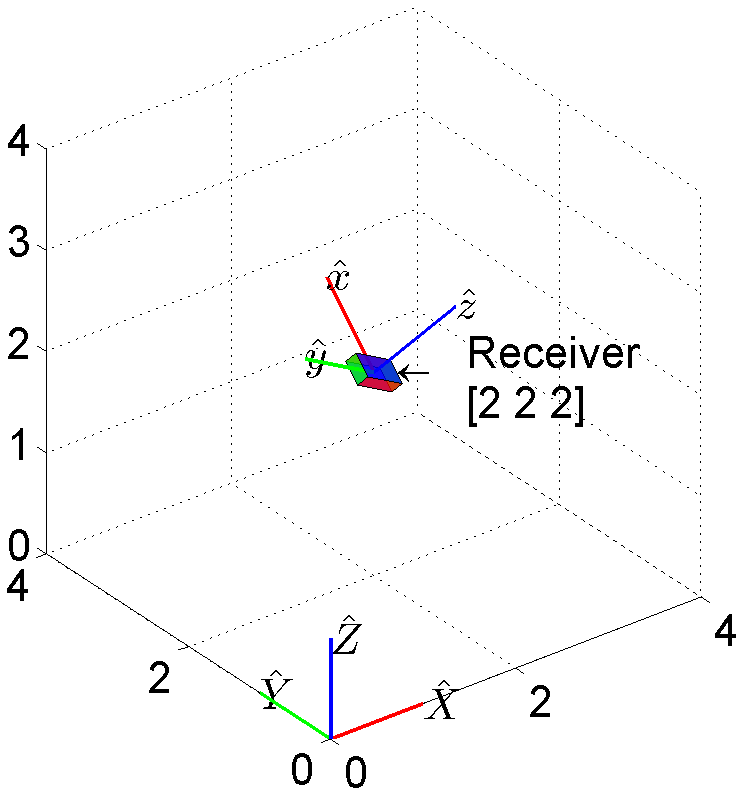
\includegraphics[trim={0.5in 0.25in 0.5in 0.25in}, clip=false, width=1.8in]{figRcvrOrientation2.png}
	%\caption{Illustration of the coordinate systems used}
	%\label{figRcvrCoord}
%\end{figure}
%
%Let [$x_{tx}$ $y_{tx}$ $z_{tx}$] be the location of centroid ($C_{tx}$) of the illumination surface of the transmitter and [$x_{rx}$ $y_{rx}$ $z_{rx}$] be the location of the centroid of the receiver concentrator surface in the GCS. The optical axis is then given by (\ref{CS0a}). The transmitter is then located at height ${\bf{d}}^{z}$ above the receiver in RCS given by (\ref{CS0b})
%\begin{subequations}
	%\begin{gather}
	%{\bf{d}} = \vectthree{x_{tx}}{y_{tx}}{z_{tx}} - \vectthree{x_{rx}}{y_{rx}}{z_{rx}} \label{CS0a}\\
	%{\bf{d}}^{z} = ({\bf{d}}.{\hat{\bf{z}}}){\hat{\bf{z}}}\label{CS0b}
%\end{gather}
%\end{subequations}

Let the radiant intensity emitted by the transmitter at any angle $\phi$ subtended between the transmitter surface normal and the optical axis be given by $L(\phi)$. Radiant intensity of a lambertian transmitter of order $m$ is given by
\begin{equation}
	\label{eqLambertian}
	L(\phi) = \twopartdef{{\frac{(m+1)}{2\pi}}cos^{m}(\phi)}{-\pi/2\leq\phi\leq\pi/2}{0}{\mbox{ else}}
\end{equation}

The SISO receiver comprises of a filter, an optical concentrator and a PD. Let $\psi$ be the angle between the receiver surface normal ($\hat{\bf{z}}$) and the optical axis. Let $\eta$ be the refractive index of the material of the concentrator and $\psi_{c}$ be the field of view of the concentrator. Then the optical concentrator gain is given by
\begin{equation}
	\label{eqOpGain}
	G(\psi) = \twopartdef{\frac{\eta^{2}}{sin^{2}(\psi_{c})}} {0\leq\psi\leq\psi_{c}\leq\frac{\pi}{2}}{0}{\psi>\psi_{c}}
\end{equation}

Let $S(\lambda)$ be the normalized SPD of the emitted radiant flux such that area under curve is 1W. Let $R(\lambda)$ be the responsivity of the PD. Let the transmission of the filter be $T(\psi,\lambda)$. Thus the effective responsivity of the receiver including the transmission and gains from all optical components is given by 
\begin{equation}
	\label{eqReff}
	R_{e}(\psi) = G(\psi)\int^{\lambda_{max}}_{\lambda_{min}}S(\lambda)T(\psi,\lambda)R(\lambda)d\lambda
\end{equation}
where $\lambda_{min}$ to $\lambda_{max}$ span all the wavelengths of interest.

If $A$ is the active area of the PD, the overall channel gain $h$ is then given by
\begin{equation}
	\label{eqChGain}
	%h = L(\phi)\frac{A}{||{\bf{d}^{z}}||^{2}}cos(\psi)R_{e}(\psi) THIS IS WRONG 
	h = L(\phi)\frac{A}{||{\bf{d}}||^{2}}cos(\psi)R_{e}(\psi)
\end{equation}

In a typical SISO VLC link, shot noise from ambient illumination dominates over that from signal \cite{bar94a}. Let $q$ be the charge of an electron. Worst cast shot noise from isotropic ambient radiant flux $P_{a}(\lambda)$ is given by
\begin{equation}
	\label{eqNshot}
	\sigma_{sh}^{2} = \frac{2qAG(\psi_{c})}{\psi_{c}}\int_{\lambda_{min}}^{\lambda_{max}}\int_{0}^{\psi_{c}}P_{a}(\lambda)R(\lambda)T(\psi,\lambda)d\psi d\lambda
\end{equation}

%A transimpedance amplifier (TIA) is generally used as the first stage amplifier in receivers. \cite{kah97a} shows how to calculate the preamplifier input noise current density. This is given by (\ref{eqNpa}). Here it is also shown that for signal bandwidths used for VLC, thermal noise dominates the preamplifier noise. This thermal noise is given by
The transimpedance amplifier (TIA) is generally the first current to voltage amplifier stage after the PD. In the absence of significant ambient illumination, the TIA noise is the dominant source of noise \cite{kah97a}. Thus shot noise from signal itself is ignored. The thermal noise from the TIA is considered as the dominant electronic noise component and is given by \cite{kah97a},
\begin{equation}
	\label{eqNpa}
	\sigma_{th}^{2} = \frac{4kT}{R_{f}}
\end{equation}
where $k$ is the Boltzmann's constant, $T$ is the absolute temperature and $R_{f}$ is the feedback resistance of the TIA.
% 5pa/rt(Hz)

Thus the total noise current density is given by
\begin{equation}
	\label{eqNoise}
	\sigma_{SISO}^{2} = \sigma_{sh}^{2} + \sigma_{th}^{2}
\end{equation}

%$E[x]$ gives the average radiant flux emitted by the transmitter
%The transmitter is constrained to emit a peak flux of $2K$. Let $B$ be the bandwidth. Then ${SNR}_{SISO}$ is defined by
%\begin{equation}
	%\label{eqSisoSNR}
	 %SNR_{SISO} = \frac{h^{2}K^{2}}{\sigma_{SISO}^{2}B} 
%\end{equation}

Using Shannon's capacity formula for a AWGN baseband channel with a transmitter constrained to power $K$ independent of illumination and bandwidth $B$, the upper bound on capacity of the SISO VLC channel is given by \cite{sha48a}
\begin{equation}
	\label{eqSisoCap}
	C_{SISO} < log_{2}\left(1 + \frac{h^{2}K}{\sigma_{SISO}^{2}B}\right)
	%C_{SISO} = log_{2}(1 + SNR_{SISO})
\end{equation}

%\footnotetext{An LED modulating at B Hz generates intensity signals band-limited in [-B B] and has signal bandwidth of 2B Hz}